%%________________________________________________________________________
%% LEIM | PROJETO
%% 2022 / 2013 / 2012
%% Modelo para relatório
%% v04: alteração ADEETC para DEETC; outros ajustes
%% v03: correção de gralhas
%% v02: inclui anexo sobre utilização sistema controlo de versões
%% v01: original
%% PTS / MAR.2022 / MAI.2013 / 23.MAI.2012 (construído)
%%________________________________________________________________________




%%________________________________________________________________________
\chapter{Sistemas de Apoio à Decisão}
\label{ch:sad}
%%________________________________________________________________________

Um \gls{sad} é uma aplicação ou conjunto de ferramentas desenhadas para ajudar os utilizadores a tomar decisões mais informadas e fundamentadas, geralmente com base na análise de dados. Na prática, um \gls{sad} recolhe, organiza e processa dados, muitas vezes em tempo real ou a partir de ficheiros carregados pelo utilizador, e apresenta esses dados de forma visual (como gráficos ou dashboards), permitindo aplicar filtros e explorar cenários. Ou seja, não toma decisões por si só, mas fornece os elementos certos para que o utilizador possa decidir melhor, especialmente em contextos complexos ou com grande volume de informação.

\chapter{Tabelas de Requisitos}
\label{ch:tabRequisitos}

\section{Requisitos Funcionais}

\begin{table}[h!]
\centering
\begin{tabular}{|l|p{7cm}|l|l|}
\hline
\textbf{Requisito} & \textbf{Função} & \textbf{Categoria} & \textbf{Agrupamento} \\
\hline
R1.1 & Permitir criação de conta - utilizador único & Visível & Autenticação \\
R1.2 & Permitir login & Visível & Autenticação \\
R2.1 & Permitir upload de ficheiros (estritamente do formato .xlsx) & Visível & Gestão de Ficheiros \\
R2.2 & Associar ficheiros carregados a trimestres & Invisível & Gestão de Ficheiros \\
R3.1 & Permitir eliminação de ficheiros carregados & Visível & Gestão de Trimestres \\
R3.2 & Permitir criação de trimestres identificados por 'Quarter N' & Visível & Gestão de Trimestres \\
R3.3 & Listar todos os trimestres do grupo & Visível & Gestão de Trimestres \\
R4.1 & Visualizar gráficos & Visível & Visualização de Dados \\
R4.2 & Aplicar filtros & Visível & Visualização de Dados \\
\hline
\end{tabular}
\caption{Tabela de Requisitos Funcionais}
\label{tab:requisitosFuncionais}
\end{table}

\section{Requisitos Não-Funcionais}

\begin{table}[h!]
    \centering
    \begin{tabular}{|l|p{7cm}|l|}
    \hline
    \textbf{Atributo} & \textbf{Detalhe / Restrição - Fronteira} & \textbf{Categoria} \\
    \hline
    Usabilidade & Detalhe - Interface intuitiva & Obrigatório \\
    Usabilidade & Detalhe - Carregamento de gráficos em sem bloquear o utilizador (lazy load) & Obrigatório \\
    Usabilidade & Detalhe - Suporte para múltiplos browsers & Obrigatório \\
    Segurança & Detalhe - Autenticação e Contas & Obrigatório \\
    Segurança & Fronteira - Cada utilizador só pode aceder aos seus dados & Obrigatório \\
    Segurança & Detalhe - Garantir que o sistema só permite ficheiros com formato previsto & Obrigatório \\
    Performance & Detalhe - Suporte para múltiplos utilizadores sem degradação significativa & Desejável \\
    Performance & Detalhe - Resposta rápida às interações do utilizador & Obrigatório \\
    Acessibilidade & Detalhe - Tem de ser navegável por teclado e screen-reader friendly & Obrigatório \\
    Dados & Normalizar os dados que recebe de forma a serem apresentáveis & Obrigatório \\

    \hline
    \end{tabular}
    \caption{Tabela de Requisitos Não Funcionais}
    \label{tab:requisitosNaofuncionais}
    \end{table}
    

\chapter{Casos de Utilização}
\label{ch:casosUtilizacao}

\begin{figure}[h]
\centering
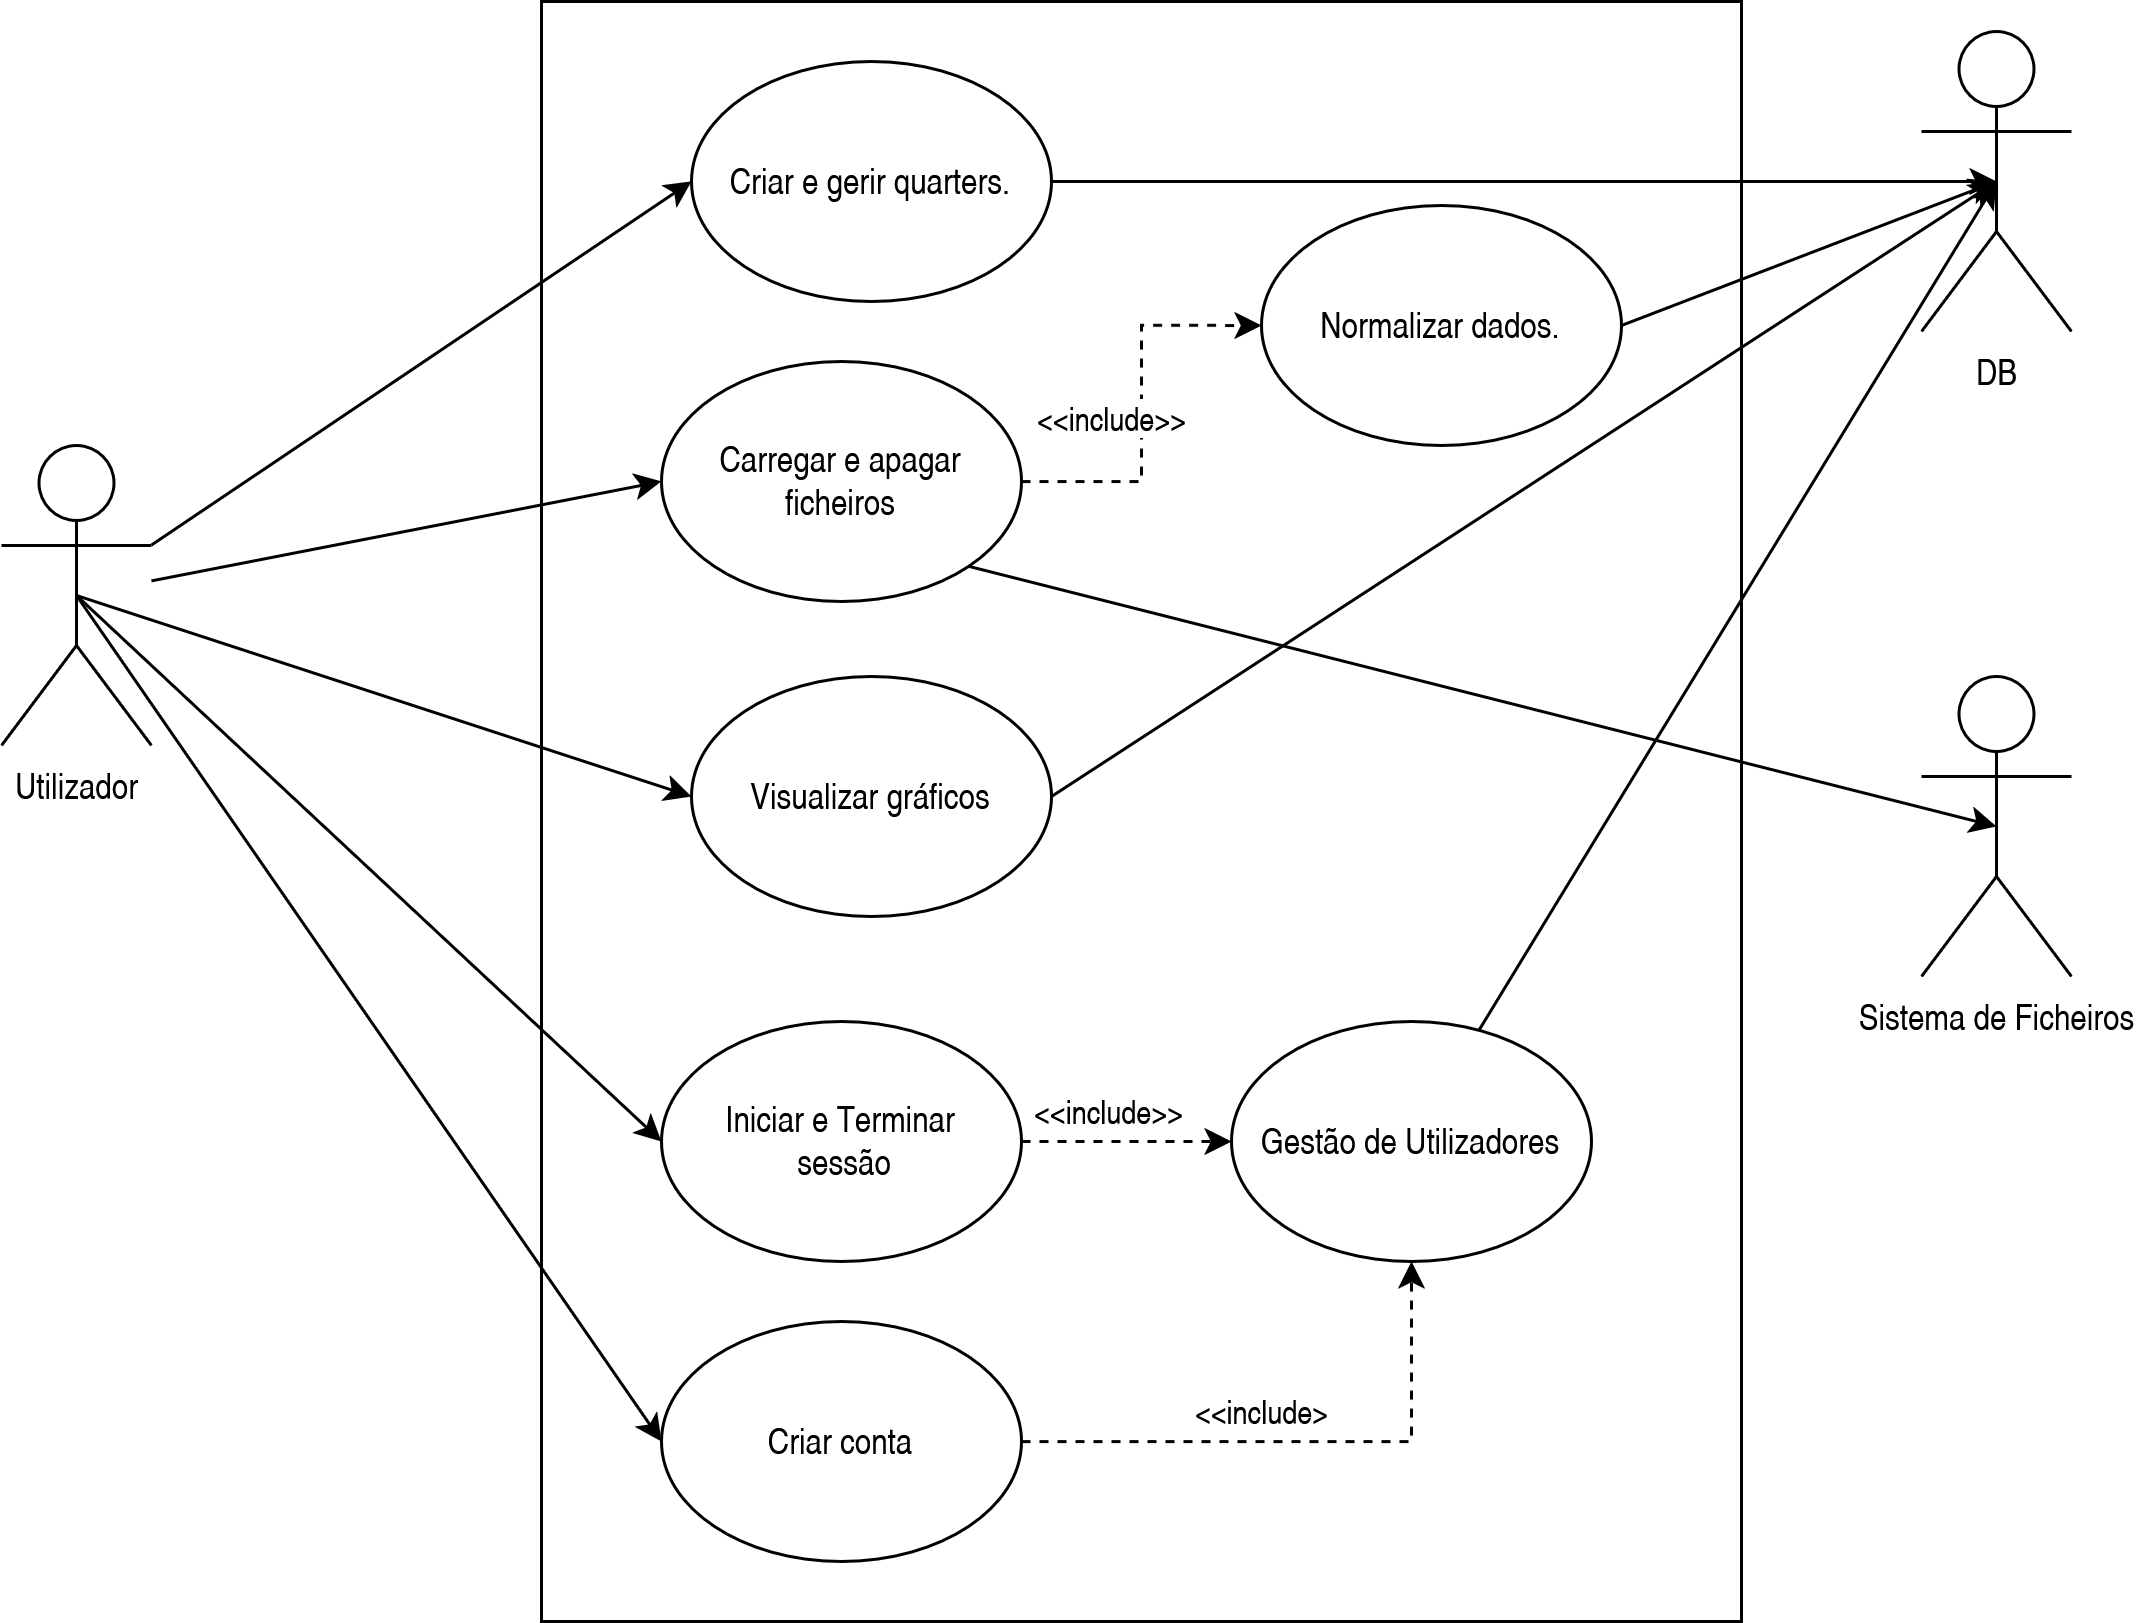
\includegraphics[width=14cm]{./img/usecase_uml}
\caption{\gls{uml} dos Casos de Utilização}
\label{fig:umlCasosUtilizacao}
\end{figure}
\textbf{ Falta a matriz de prioridade dos casos de utilização}


\chapter{Classificação das folhas \gls{xlsx}}
\label{ch:asd}









